\documentclass{article}
\usepackage[utf8]{inputenc}
\usepackage{xurl}
\usepackage[czech]{babel}
\usepackage{csquotes}
\usepackage{dcolumn}
\usepackage{subfig}
\usepackage{graphicx}

\MakeOuterQuote{"}

\title{Metody analýzy dat I - analýza datasetu}
\author{Filip Peterek, PET0342}
\date{28. prosinec 2021}

\begin{document}

\maketitle

\section{Popis datové sady}

Datová sada obsahuje seznam nahlášených zločinů za rok 2018 ve městě Austin
v americkém státě Texas. Data byla sbírána policií města Austin a následně
veřejně publikována \cite{dataset-source}. Datová sada obsahuje 37156 záznamů
odpovídajících 37156 nahlášeným zločinům.

\subsection{Atributy datové sady}

V datové sadě se objevuje 13 atributů, které jsou popsány v následující tabulce.

\begin{table}
  \centering
  \caption{Popis atributů datové sady}
  \begin{tabular}{ |l|l|l|l|l| }
  \hline
    Název & Popis & Typ & Datový typ & Povinný \\
    GO Primary Key & ID incidentu & numerický & celé číslo & ano \\
    Council District & městská čtvrť & kategoriální & celé číslo & ne \\
    GO Highest Offense & zločin & kategoriální & řetězec & ano \\
    Crime Type & typ zločinu & kategoriální & řetězec & ano \\
    GO Report Date & den nahlášení & numerický & datum & ano \\
    GO Location & místo odehrání zločinu & kategoriální & řetězec & ne \\
    GO X Coordinate & místo odehrání zločinu & numerický & desetinné číslo & ne \\
    GO Y Coordinate & místo odehrání zločinu & numerický & desetinné číslo & ne \\
    Clearance Status & stav policejního pátrání & kategoriální & řetězec & ne \\
    Clearance Date & datum vyřešení případu & numerický & datum & ne \\
    GO District & policejní sektor & kategoriální & řetězec & ano \\
    GO Location Zip & poštovní směrovací číslo & kategoriální & celé číslo & ne \\
    GO Census Tract & čtvrť podle počtu obyvatel & kategoriální & desetinné číslo & ne \\
  \hline
  \end{tabular}
\end{table}

\section{Výsledky analýzy}

\subsection{Počty zločinů}

Počty jednotlivých zločinů \ref{fig:crime_counts} jistě nijak zarážející nejsou. Naprosto
převažují krádeže, v tomto případě se z velké části pravděpodobně jedná hlavně o kapsářství
a podobné drobné krádeže. Počet vloupání do domu je oproti obyčejným kráděžím méně
než pětinový. Násilné činy tak časté nejsou, přesto se jich několik objevuje.

\begin{figure}
  % \centering
  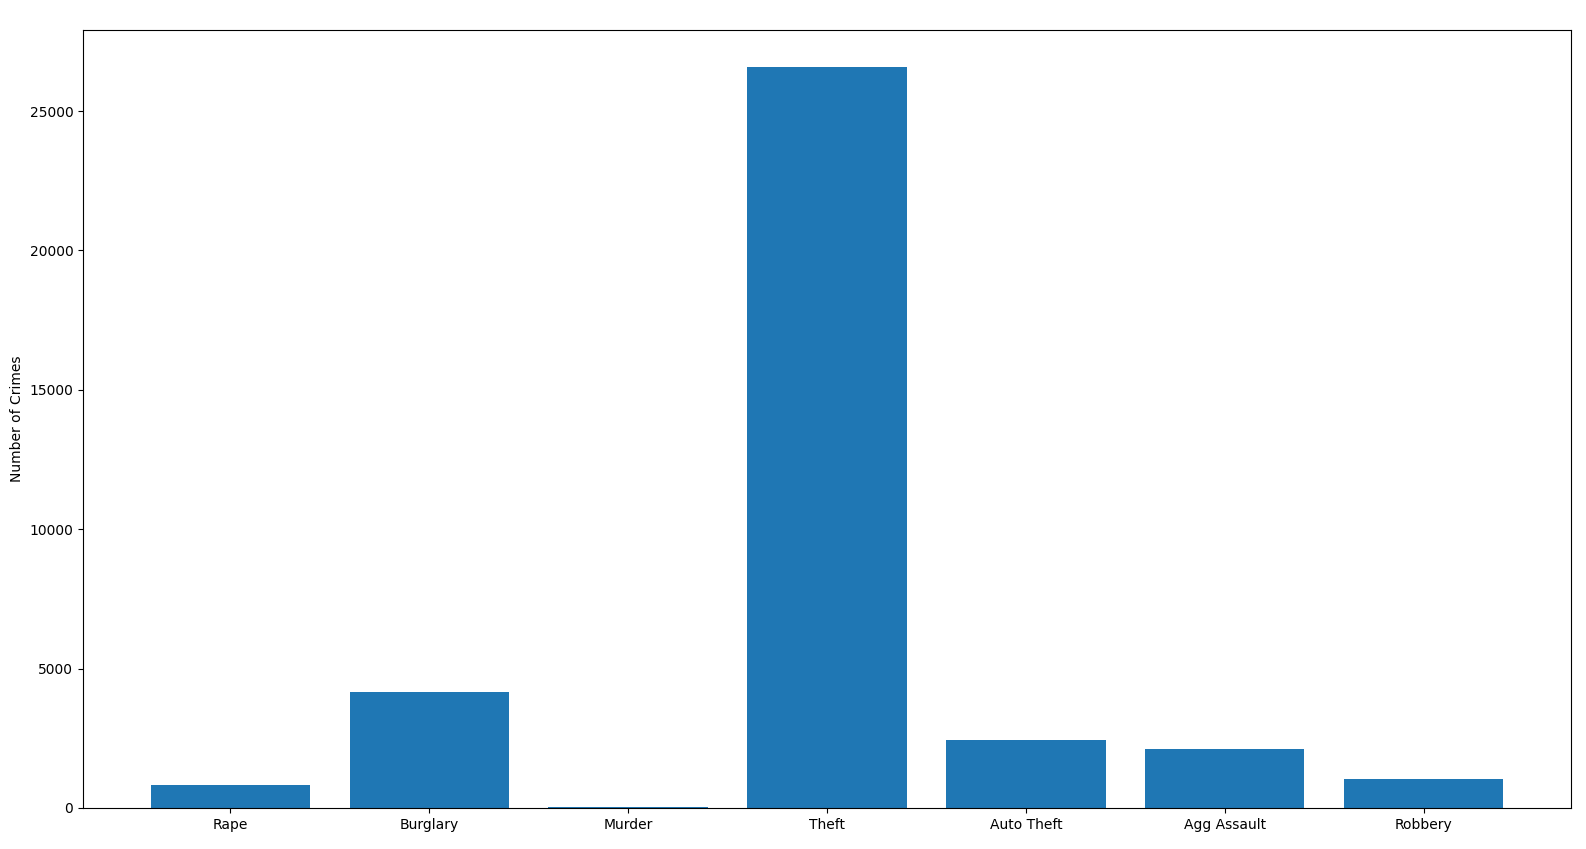
\includegraphics[width=1.4\textwidth]{figures/crime_counts.png}
  \caption{Počet nahlášených zločinů podle kategorie}
  \label{fig:crime_counts}
\end{figure}

Velmi znepokojující jsou počty nahlášeného násilí na dětech \ref{fig:crime_against_children}.
Austin je velké město, a proto se s vysokou pravděpodobností objeví zločiny všech možných typů,
přesto řádově stovky případů zneužívání dětí je alarmující číslo.

\begin{figure}
  \centering
  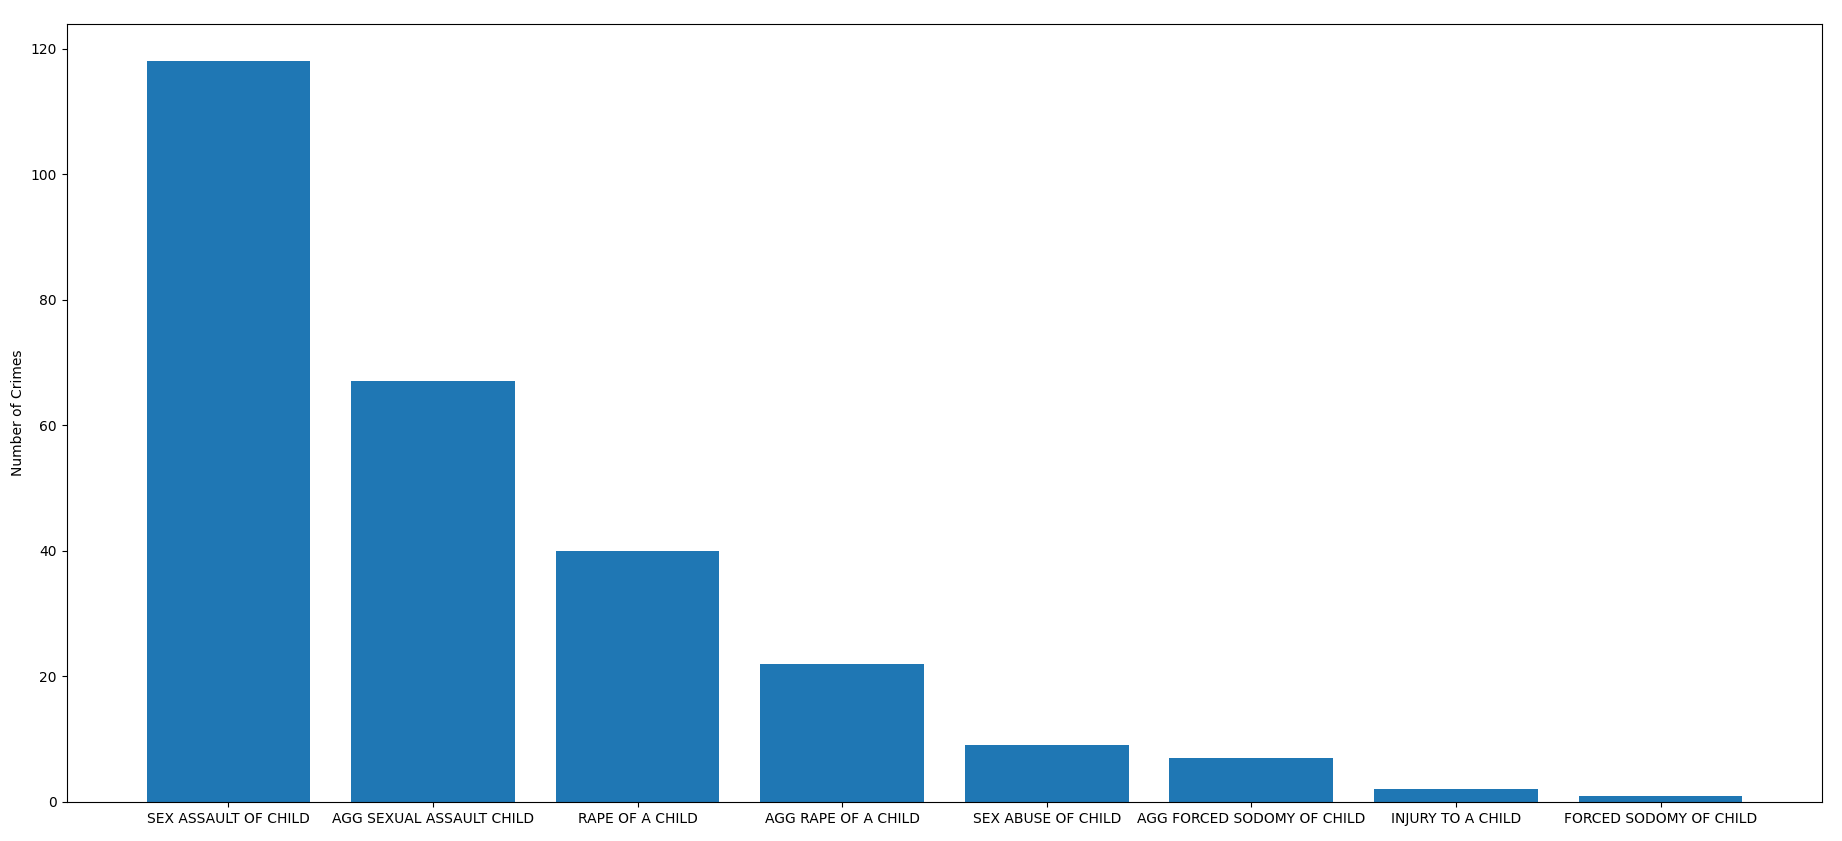
\includegraphics[width=1.4\textwidth]{figures/crime_against_children.png}
  \caption{Počet nahlášených zločinů proti dětem}
  \label{fig:crime_against_children}
\end{figure}

Počet nahlášených zločinů podle kalendářního měsíce \ref{fig:crime_per_each_month} není
nijak zajímavý. Nejméně zločinů bylo nahlášeno v únoru -- nepřekvapivě, neboť se jedná
o nejkratší měsíc v roce. Nejvíce zločinů bylo nahlášeno v říjnu. Překvapivě může působit
fakt, že nedošlo k nárůstu zločinnosti v letních měsících. Austin sice nepatří mezi
nejvyhledávanější turistické destinace ve Spojených státech, přesto se však jedná o město
s bohatým kulturním vyžitím. I tak ale nedošlo k nárůstu zločinnosti v letních měsících.

\begin{figure}
  \centering
  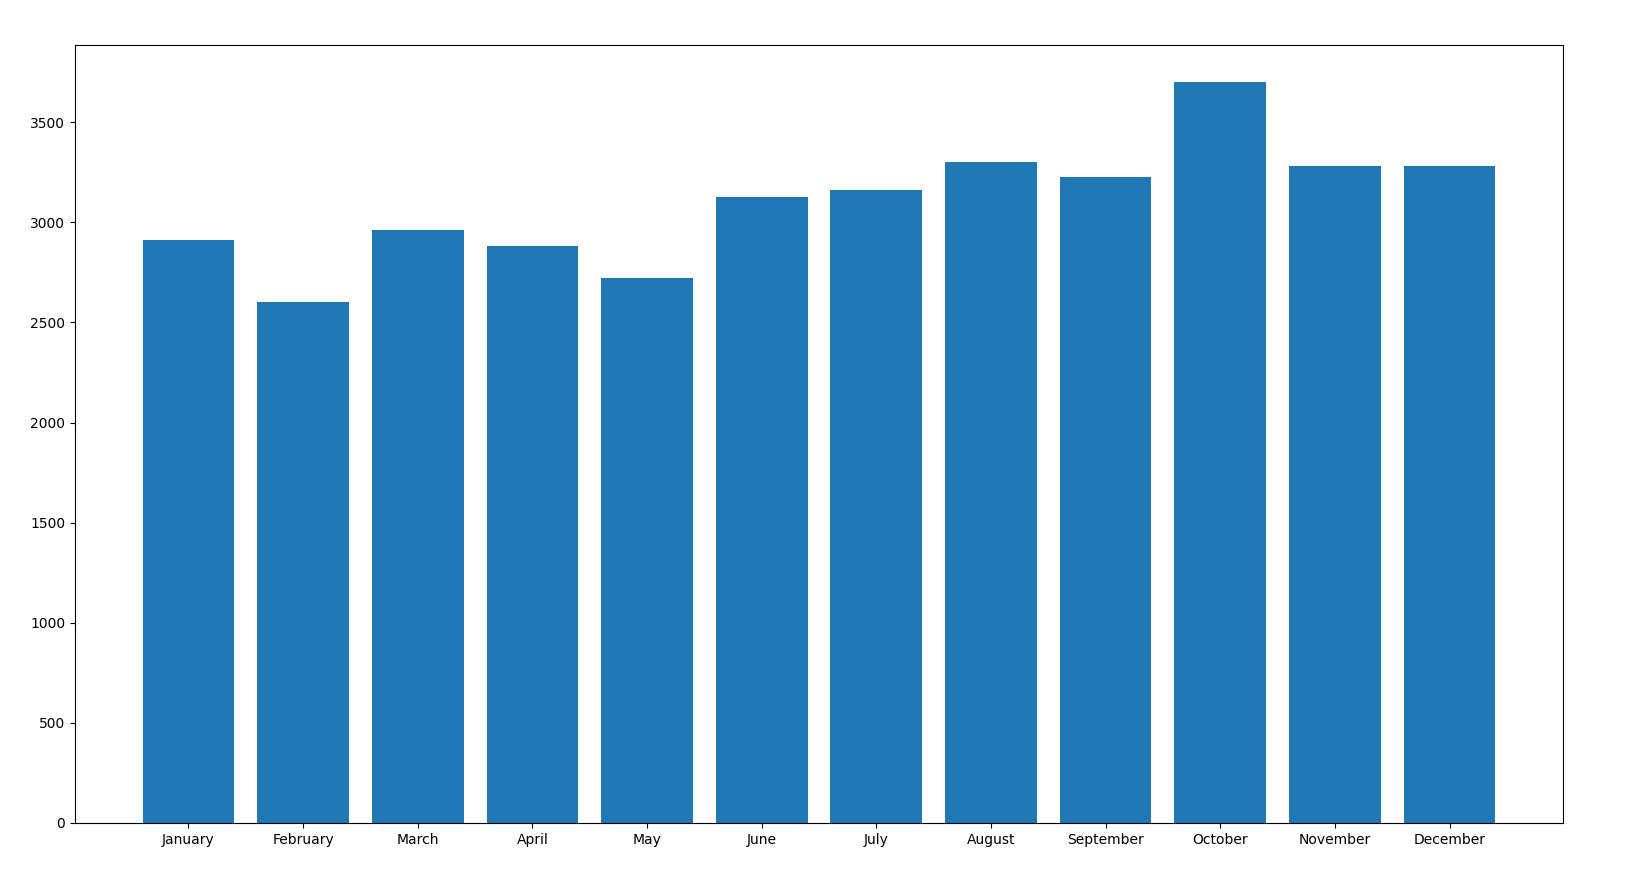
\includegraphics[width=1.4\textwidth]{figures/crime_per_each_month.png}
  \caption{Počet nahlášených zločinů podle kalendářního měsíce}
  \label{fig:crime_per_each_month}
\end{figure}

Drobný nárůst zločinnosti v říjnu může vzbudit určitou zvědavost, při podrobnějším prozkoumání
ovšem zjistíme, že se neobjevily žádné zajímavé zločiny (např. hromadné nahlášení daňových úniků),
jednalo se převážně o drobné krádeže. Přesto tato skutečnost může být zajímavá pro policejní
oddělení města Austin.

\begin{figure}
  \centering
  \includegraphics[width=1.4\textwidth]{figures/october_crime.png}
  \caption{Sedm nejčastějších zločinů v říjnu 2018}
  \label{fig:october_crime}
\end{figure}

\subsection{Řešení zločinů}

Vzorného občana určitě znepokojí množství nevyřešených příkladů. Z grafu \ref{fig:clearance_status}
lze vyčíst, že naprostá většina případů zůstáva nevyřešena.

\begin{figure}
  \centering
  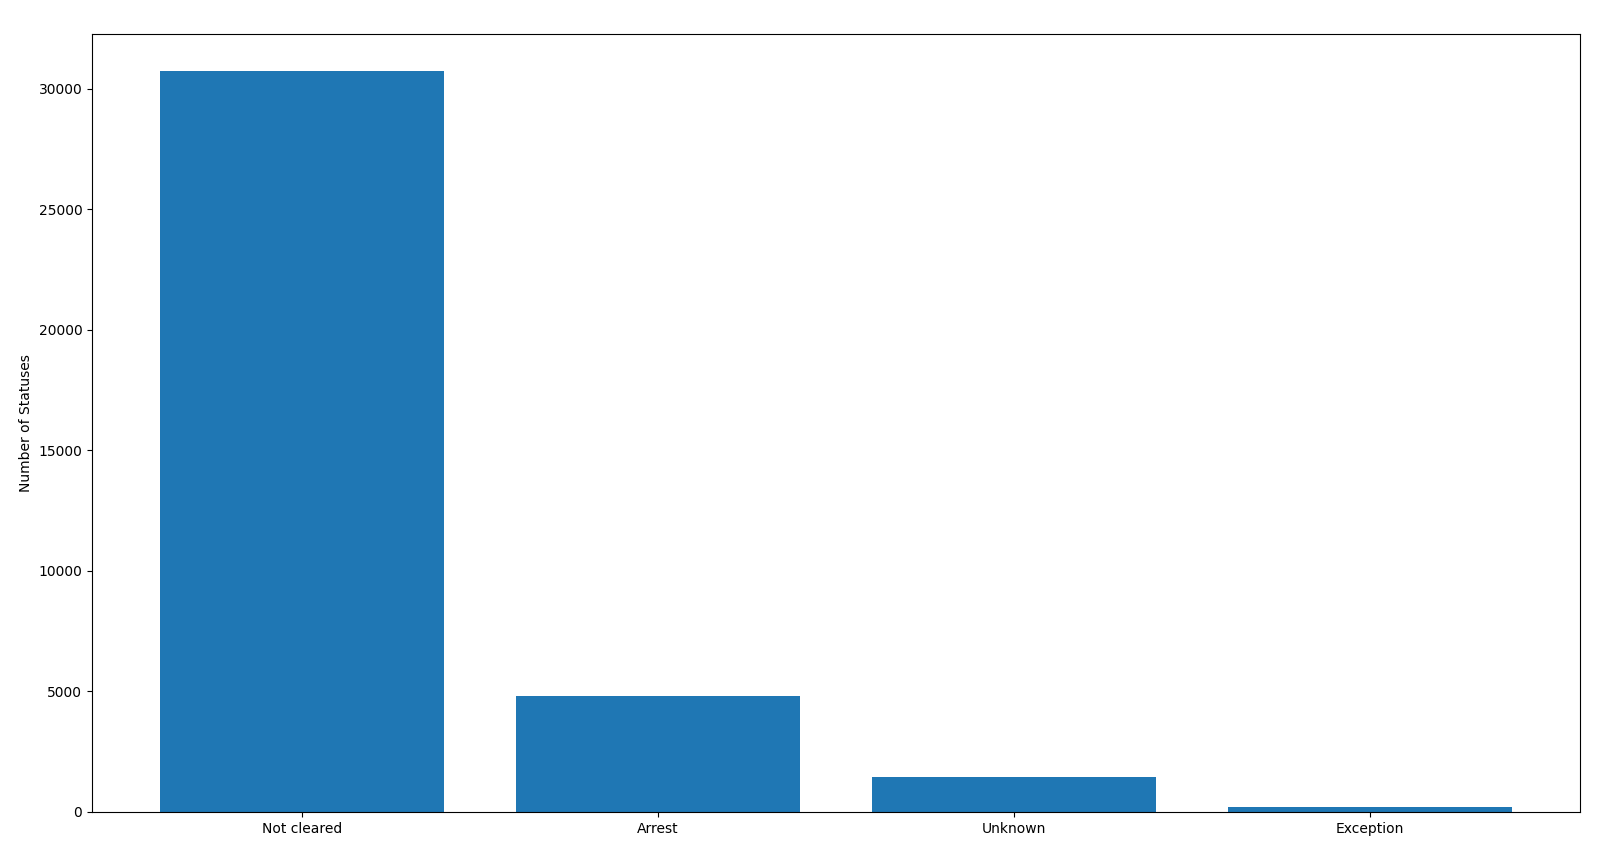
\includegraphics[width=1.4\textwidth]{figures/clearance_status.png}
  \caption{Četnosti statusů policejního pátrání}
  \label{fig:clearance_status}
\end{figure}

Z grafu průměrné délky řešení případu \ref{fig:clearance_time} zjistíme, že nejkratší dobu trvá
řešení krádeží. Graf znázorňuje pouze úspěšně vyřešené případy. Nejrychleji jsou v průměru řešeny
krádeže. Nejdéle jsou řešeny případy znásilnění, jejichž řešení trvá v průměru přes 80 dní.
Možná překvapivě jsou případy vražd a zabití vyřešeny v průměru do jednoho měsíce.

\begin{figure}
  \centering
  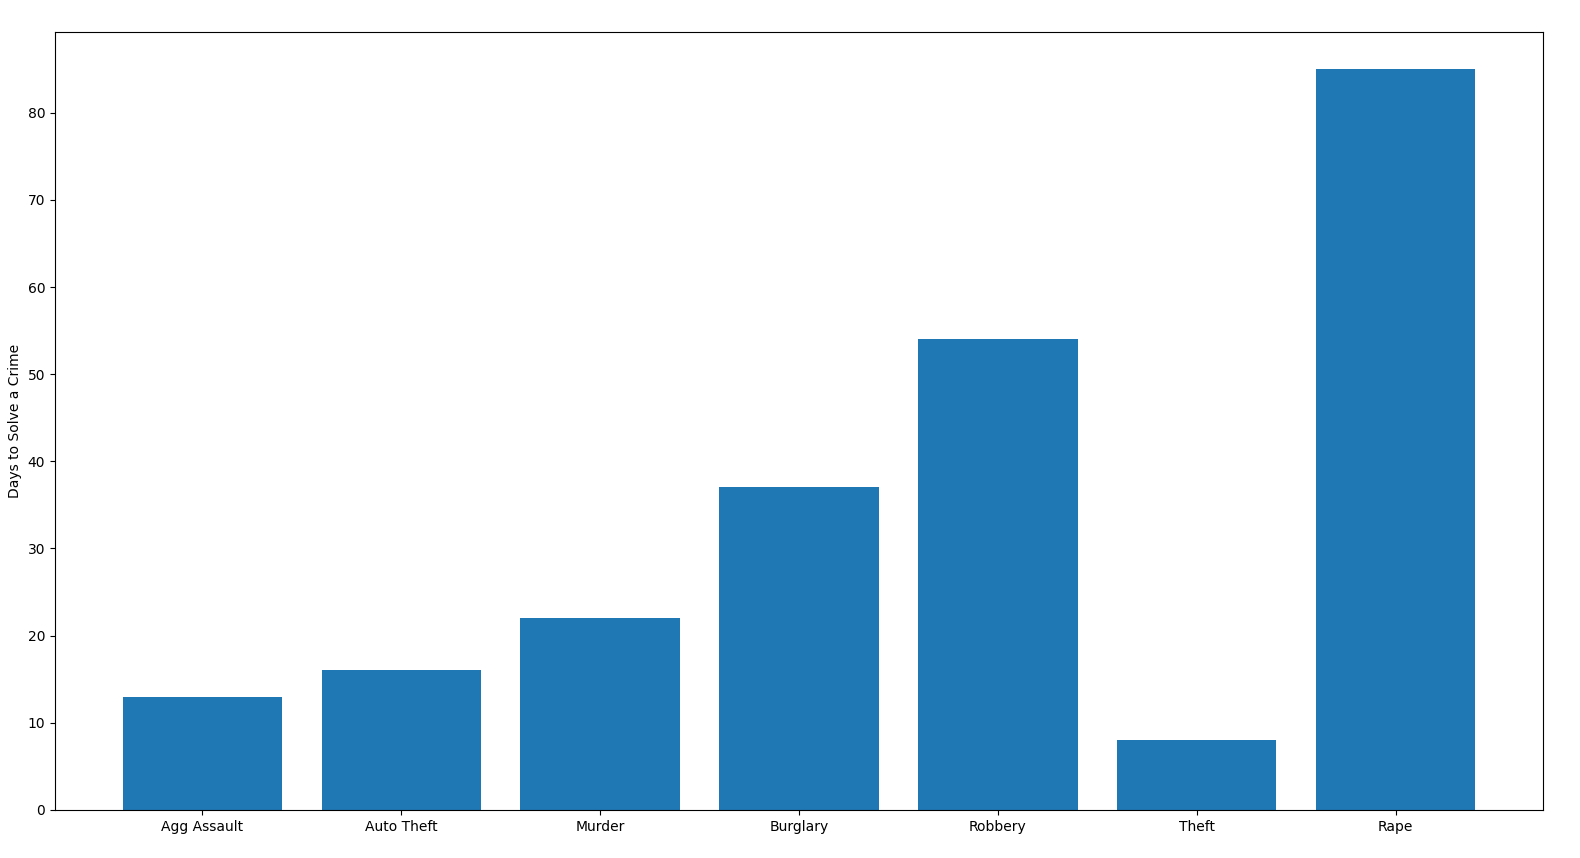
\includegraphics[width=1.4\textwidth]{figures/clearance_time.png}
  \caption{Průměrná doba úspěšného řešení}
  \label{fig:clearance_time}
\end{figure}

Pokud se podíváme na pět nejdéle řešených případů \ref{fig:top_clearance_times}, zjistíme, že byly
všechny řešeny déle než rok. Jinak ale nezjistíme žádný zajímavější trend, mezi nejdéle řešenými
případy najdeme různé typy zločinů. Překvapivě působí pouze fakt, že jsou délky řešení případů
daleko za průměrem úspěšného řešení konkrétního typu zločinu.

Ovšem podíváme-li se na průměrnou délku řešení případu, medián délky, a varianci
\ref{tab:avg_clearance} (včetně uzavření nevyřešených případů), zjistíme, že průměr (a ani medián),
nejsou příliš vypovídající.

\begin{table}
  \centering
  \caption{Délka řešení případu}
  \label{tab:avg_clearance}
  \begin{tabular}{ |l|l| }
  \hline
      Průměr & 16.0 \\
      Medián & 8.0 \\
      Variance & 1172 \\
  \hline
  \end{tabular}
\end{table}

\begin{figure}
  \centering
  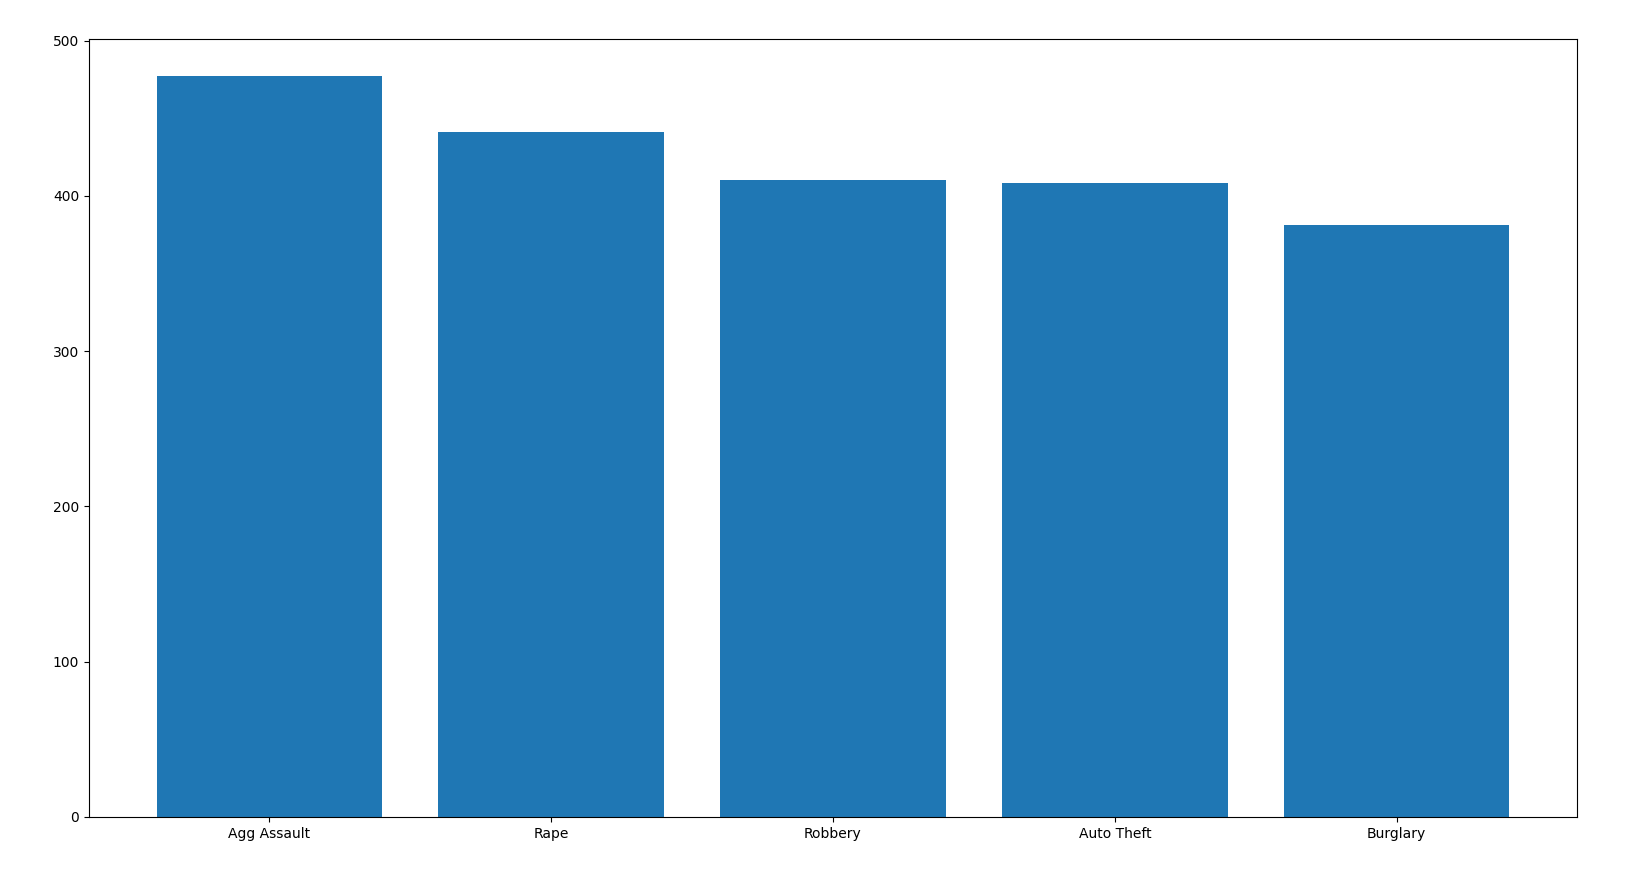
\includegraphics[width=1.4\textwidth]{figures/top_clearance_times.png}
  \caption{Nejdéle řešené jednotlivé případy}
  \label{fig:top_clearance_times}
\end{figure}

Počty uzavřených případů podle kalendářního měsíce \ref{fig:clearance_by_month} převážně kopírují
počty nahlášených případů. Nejvíce případů bylo uzavřeno v říjnu a listopadu, což pouze reflektuje
fakt, že bylo v říjnu nahlášeno nejvíce případů -- z velké části se jednalo převážně o drobné krádeže,
které jsou zpravidla uzavírány velmi rychle. Nejméně případů bylo vyřešeno v únoru. Tato informace
je také nepřekvapivá, jelikož se jedná o nejkratší měsíc v roce.

\begin{figure}
  \centering
  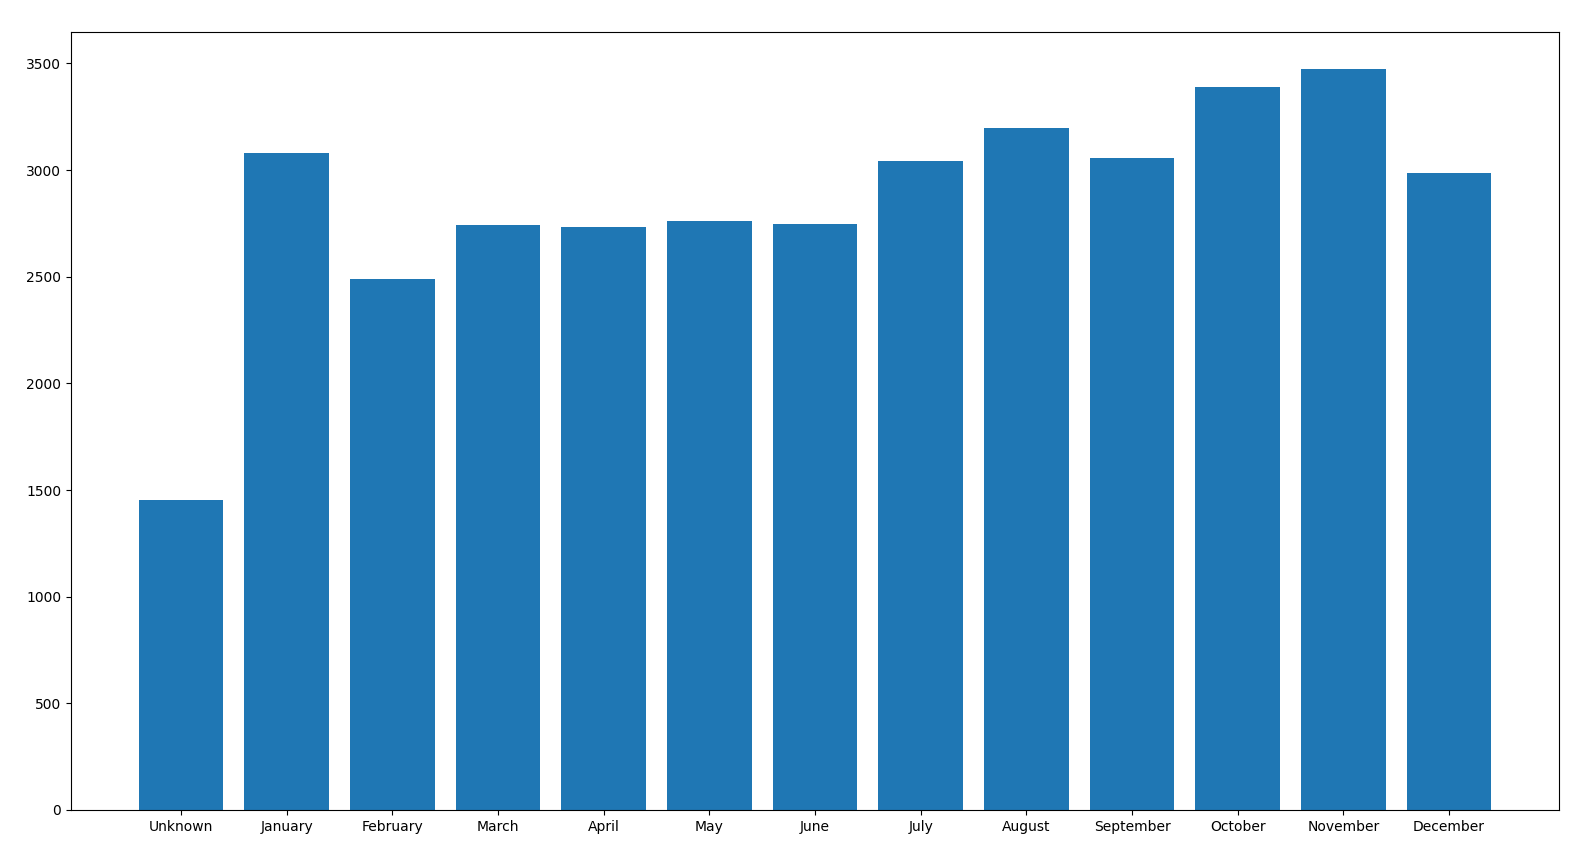
\includegraphics[width=1.4\textwidth]{figures/clearance_by_month.png}
  \caption{Počet uzavřených případů podle kalendářního měsíce}
  \label{fig:clearance_by_month}
\end{figure}

Děsivě může působit poměr vyřešených případů v poměru k celkovému počtu případů
\ref{fig:solved_percentage}. Méně než pětina vloupání, přibližně pětina krádeží aut, a přibližně
čtvrtina znásilnění skončila úspěšným vyřešením případu (zatčením pachatele nebo výjimečným řešením).
Statistika násilných napadení je poněkud lepší, více než polovina případů skončila úspěšným vyřešením.
Nejlepší statistiku nalezneme u zabití (ať už úmyslných nebo neúmyslných). 27 z celkového počtu 32, tedy
přes 80 \% případů zabití skončilo nalezením pachatele. Z grafu tedy vyplývá, že trváte-li nutně na dopadení
pachatele, musíte se nechat zavraždit.

\begin{figure}
  \centering
  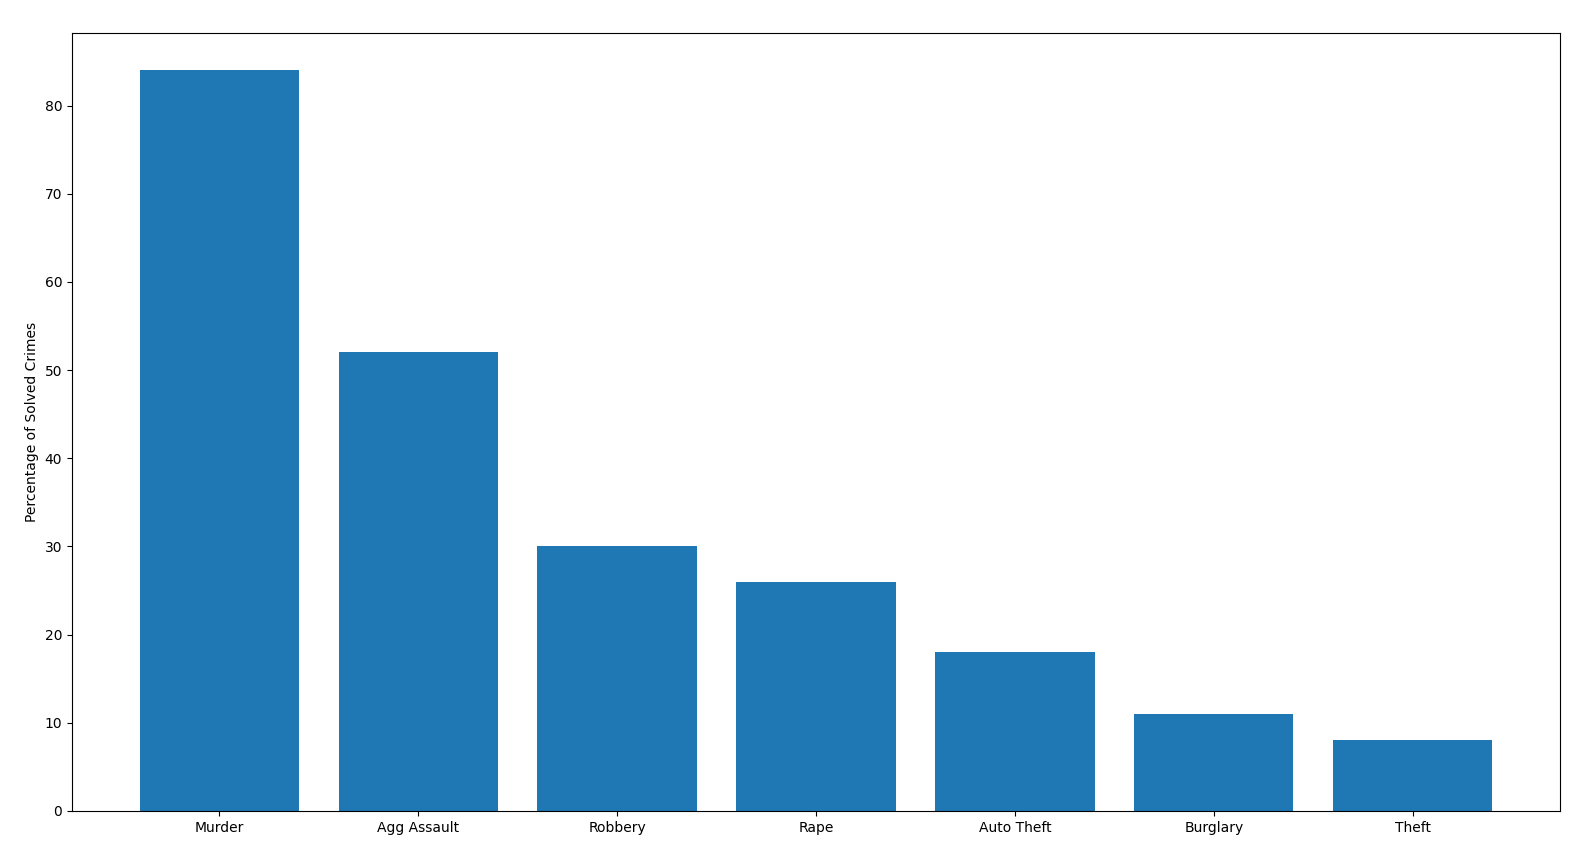
\includegraphics[width=1.4\textwidth]{figures/solved_percentage.png}
  \caption{Poměr úspěšně vyřešených případů (v procentech)}
  \label{fig:solved_percentage}
\end{figure}

\subsection{Bezpečnost městských částí}

Případného návštěvníka města Austin může zajímat statistika nejméně bezpečných ulic \ref{fig:worst_streets}.
Při bližším prozkoumání však zjistíme, že ty nejméně bezpečné ulice jsou zároveň jedny z nejdelších ulic
v Austinu, a jedná se o ulice, které se většinou táhnou přes polovinu města.

\begin{figure}
  \centering
  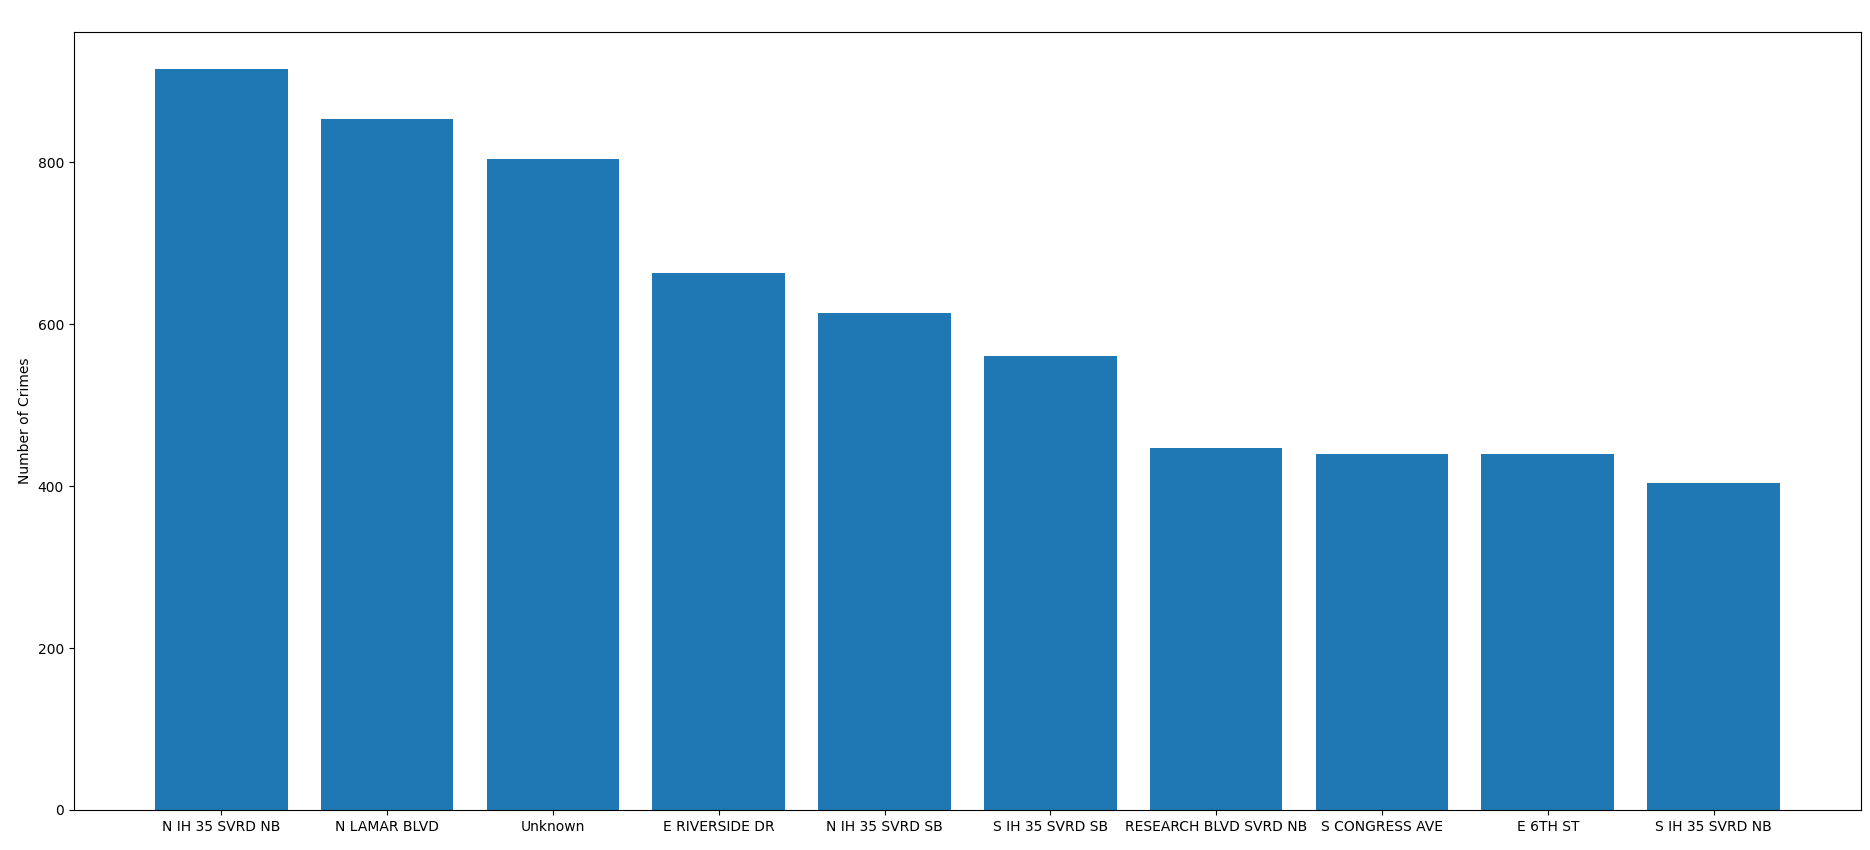
\includegraphics[width=1.4\textwidth]{figures/worst_streets.png}
  \caption{Ulice s nejvyšším počtem nahlášených zločinů}
  \label{fig:worst_streets}
\end{figure}

Z charakteristiky datové sady vyplývá, že datová sada nebude obsahovat ulice, na kterých k žádnému
zločinu nedošlo. Mezi ulicemi, na kterých byl nahlášen alespoň jeden zločin, najdeme spoustu ulic,
kde došlo k nahlášení právě jednoho zločinu \ref{fig:safest_streets}. Proto statistika nejbezpečnějších
ulic není příliš vypovídající.

\begin{figure}
  \centering
  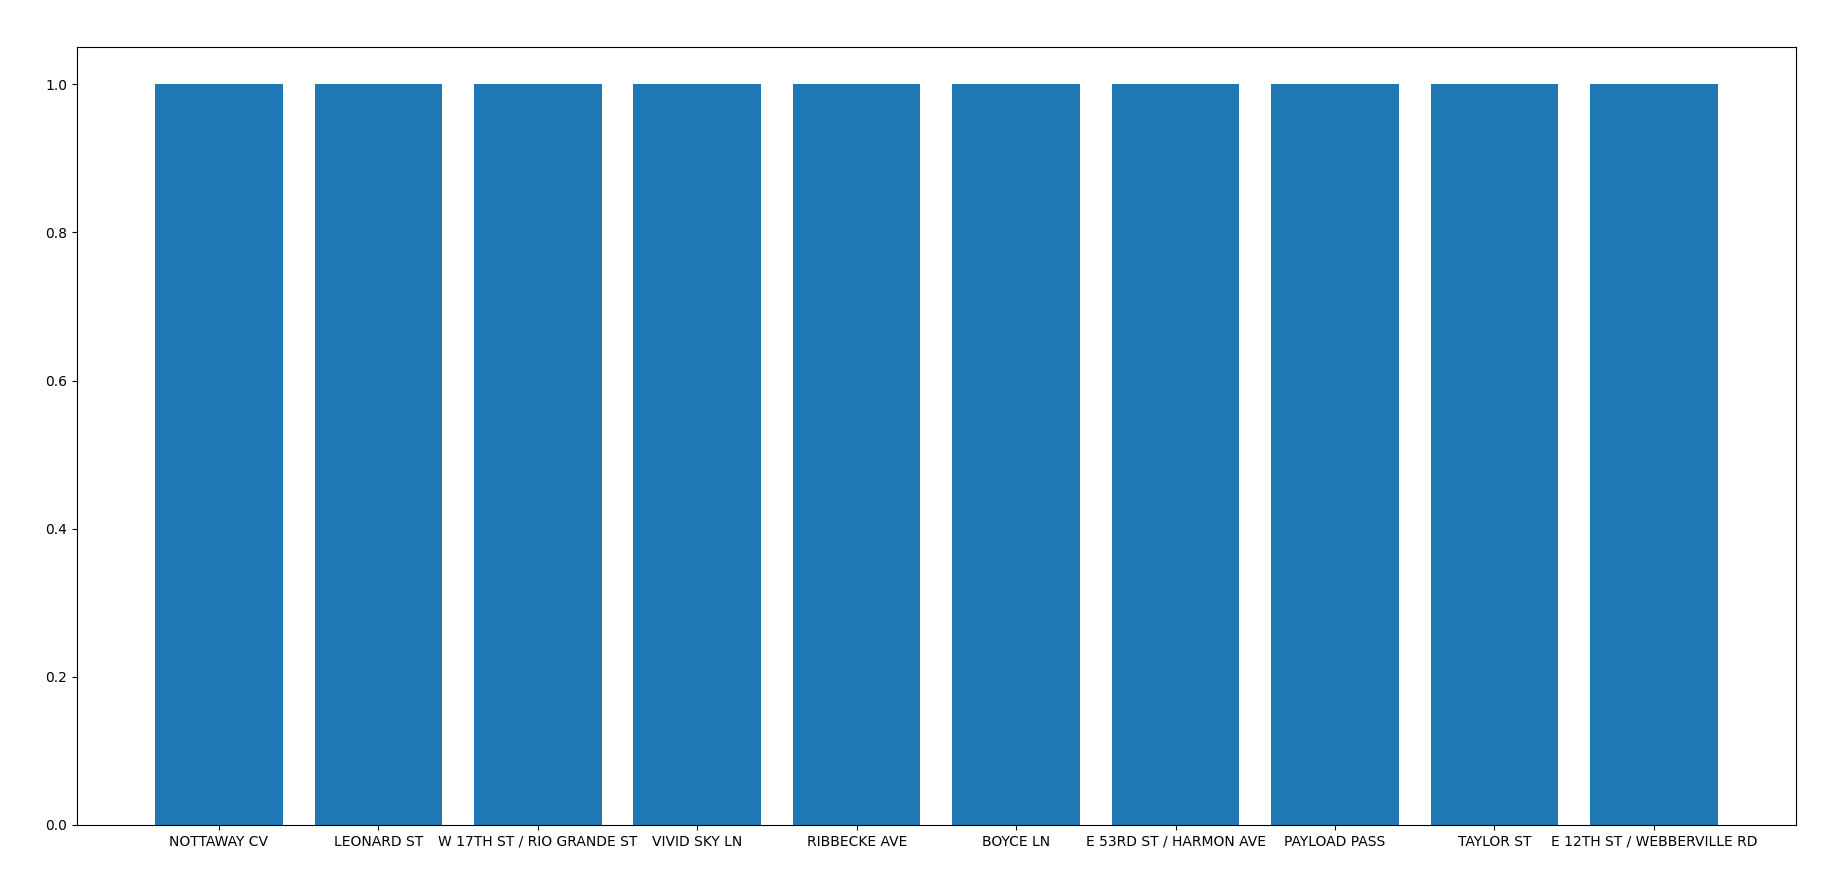
\includegraphics[width=1.4\textwidth]{figures/safest_streets.png}
  \caption{Ulice s nejnižším počtem zločinů (ulice bez zločinů jsou ignorovány)}
  \label{fig:safest_streets}
\end{figure}

Zákony dodržujícího občana bude zajímat také seřazení čtvrtí podle bezpečnosti. Nejméně bezpečnou čtvrtí
je čtvrť číslo devět. Čtrvť číslo devět je ovšem také centrum města Austin. Nejbezpečnějšími čtvrtěmi jsou
poté čtvrti šest, osm a deset. V případě těchto čtvrtí se zase jedná o odlehlejší a klidnější čtvrti.
\ref{austin-districts}

\begin{figure}
  \centering
  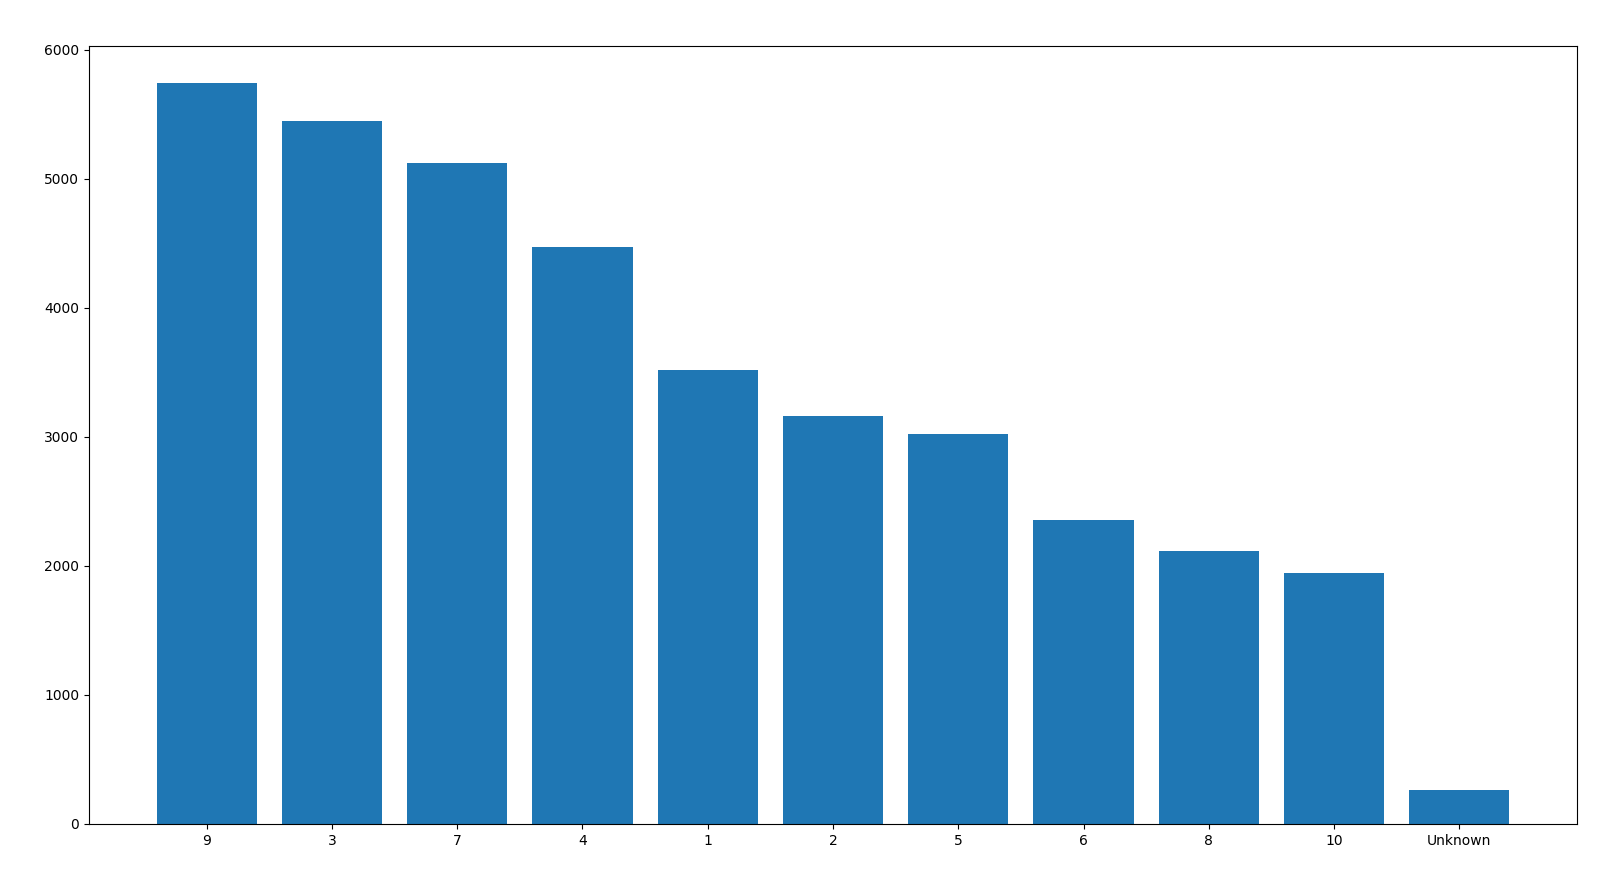
\includegraphics[width=1.4\textwidth]{figures/worst_districts.png}
  \caption{Čtvrti seřazené podle počtu nahlášených zločinů}
  \label{fig:worst_districts}
\end{figure}

\subsection{Slaughter lane}

Určitou kuriozitou je existence ulice s názvem \emph{Slaughter Lane}. Opět se jedná o relativně dlouhou ulici,
proto nikoho nemůže překvapit vyšší počet nahlášených zločinů. Kuriózní je ovšem fakt, že na východní ani západní
\emph{Slaughter Lane} nebyla nahlášena ani jedna vražda nebo zabití. Lze tedy říct, že se jedná o tzv.
false advertising a ulice \emph{Slaughter Lane} si své jméno nezaslouží.

\begin{figure}
  \centering
  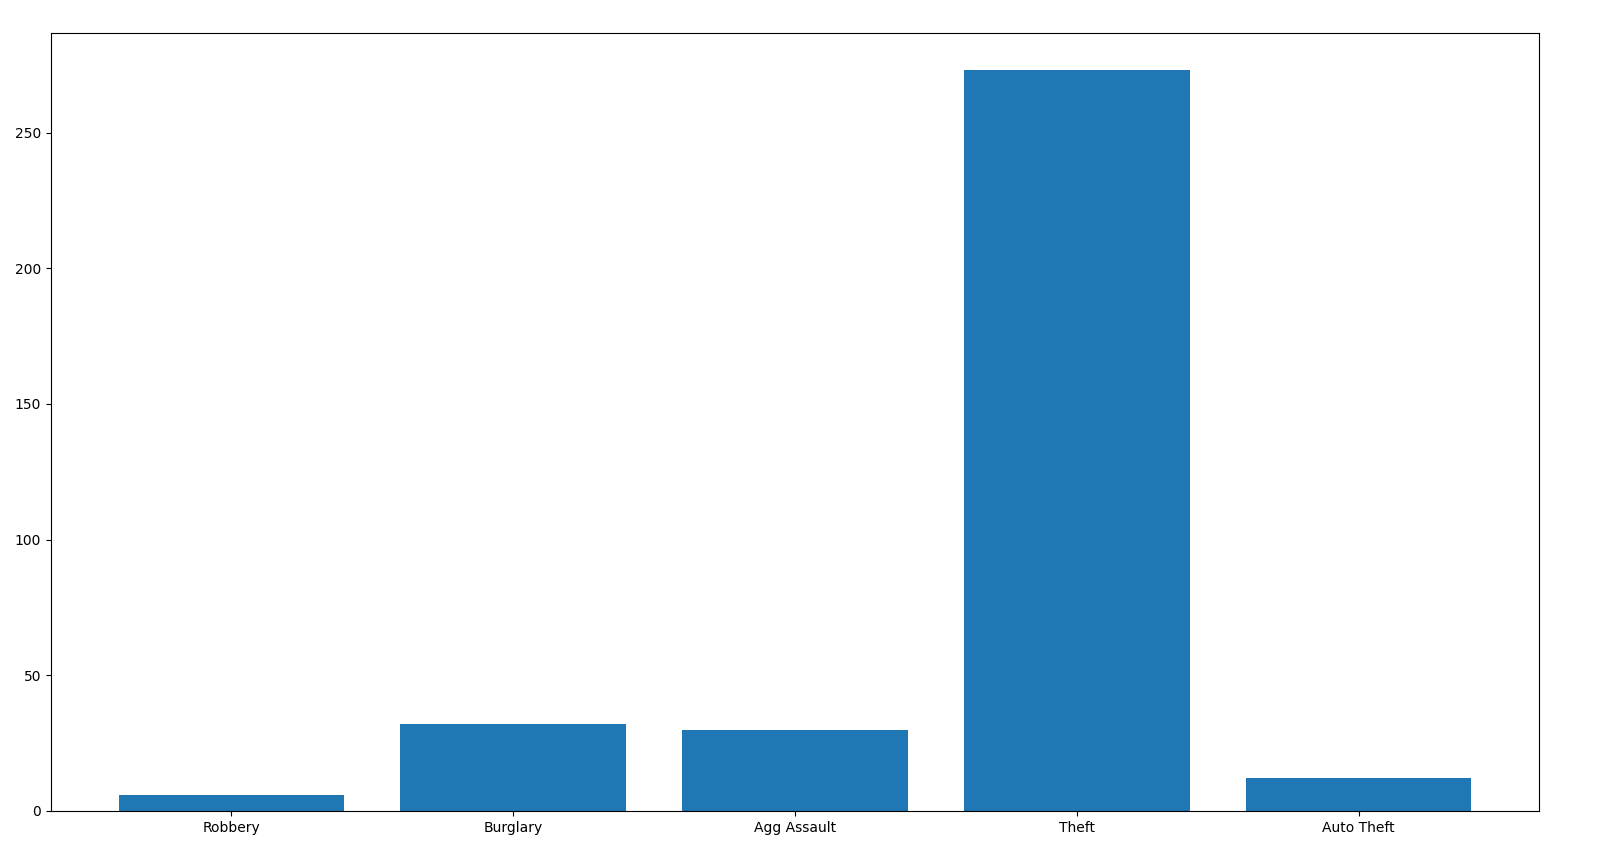
\includegraphics[width=1.4\textwidth]{figures/slaughter_lane.png}
  \caption{Četnosti zločinů na ulici Slaughter lane}
\end{figure}

\begin{thebibliography}{50}

\bibitem{dataset-source}
City of Austin \textit{2018 Annual Crime} [online, cit. 2021-12-28]
Dostupné z: \url{https://data.austintexas.gov/Public-Safety/2018-Annual-Crime/pgvh-cpyq} 
City of Austin, 6. leden 2020

\bibitem{austin-districts}
City of Austin \textit{Council District Map} [online, cit. 2021-12-29]
Dostupné z: \url{https://www.austintexas.gov/GIS/CouncilDistrictMap/} 
City of Austin

\end{thebibliography}

\end{document}

